\begin{question}
\noindent Triangle $T$ is drawn on the grid below. The line $x = 2$ is also shown.

\begin{center}
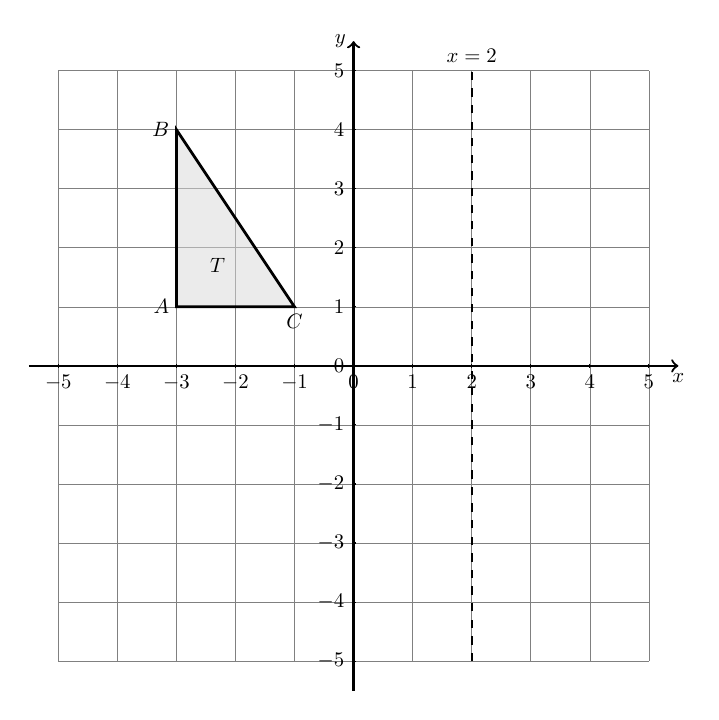
\begin{tikzpicture}[scale=0.75, transform shape]
    % Define colours
    \definecolor{borderColour}{HTML}{000000}
    \definecolor{fillColour}{HTML}{D8D8D8}

    % Define axis scale
    \def\axisLimit{5}

    % Draw grid
    \draw[step=1cm,gray,very thin] (-\axisLimit,-\axisLimit) grid (\axisLimit,\axisLimit);

    % Draw axes
    \draw[thick,->] (-\axisLimit-0.5,0) -- (\axisLimit+0.5,0) node[anchor=north] {$x$};
    \draw[thick,->] (0,-\axisLimit-0.5) -- (0,\axisLimit+0.5) node[anchor=east] {$y$};

    % Label x-axis and y-axis
    \foreach \x in {-\axisLimit,...,\axisLimit}
        \draw (\x cm,1pt) -- (\x cm,-1pt) node[anchor=north] {$\x$};
    \foreach \y in {-\axisLimit,...,\axisLimit}
        \draw (1pt,\y cm) -- (-1pt,\y cm) node[anchor=east] {$\y$};

    % Draw the mirror line x = 2
    \draw[thick,dashed] (2,-5) -- (2,5) node[anchor=south] {$x=2$};

    % Define coordinates for the vertices of triangle T
    \coordinate (A) at (-3,1);
    \coordinate (B) at (-3,4);
    \coordinate (C) at (-1,1);

    % Draw the original triangle
    \filldraw[fill=fillColour, draw=borderColour, line width=1pt, fill opacity=0.5] (A) -- (B) -- (C) -- cycle;

    % Label the vertices of the original triangle
    \node[left] at (A) {$A$};
    \node[left] at (B) {$B$};
    \node[below] at (C) {$C$};
    \node at (-2.3,1.7) {$T$};

\end{tikzpicture}
\end{center}

\noindent Reflect triangle $T$ in the line $x = 2$.

\vspace{4cm}

\begin{flushright}
    \answermarks{2}
\end{flushright}
\end{question}
